%%%%%%%%%%%%%%%%%%%%%%%%%%%%%%%%%%%%%%%%%%%%%%%%%%%%%%%%%%%%%%%%%%%%%%%%%%%%%%%%
%2345678901234567890123456789012345678901234567890123456789012345678901234567890
%        1         2         3         4         5         6         7         8


\documentclass[letterpaper, 10 pt, conference]{ieeeconf}  % Comment this line out
                                                          % if you need a4paper
%\documentclass[a4paper, 10pt, conference]{ieeeconf}      % Use this line for a4
                                                          % paper

\IEEEoverridecommandlockouts                              % This command is only
                                                          % needed if you want to
                                                          % use the \thanks command
\overrideIEEEmargins
% See the \addtolength command later in the file to balance the column lengths
% on the last page of the document

\usepackage{graphicx}
\usepackage{float}
\usepackage{graphics}
\usepackage[utf8]{inputenc}
%\usepackage[spanish, activeaccute]{babel} %permite escribir con ortografía en español, acentos, ñ, etc
\usepackage[spanish,es-noshorthands]{babel}
\usepackage{mathtools} %matematica
\usepackage{amsmath} %matematica
\usepackage{circuitikz} %pa dibujar circuitoz
\usepackage{siunitx} %simbologia, ohm etc


% Para los acentos
%\usepackage[spanish]{babel}
% The following packages can be found on http:\\www.ctan.org
%\usepackage{graphics} % for pdf, bitmapped graphics files
%\usepackage{epsfig} % for postscript graphics files
%\usepackage{mathptmx} % assumes new font selection scheme installed
%\usepackage{times} % assumes new font selection scheme installed
%\usepackage{amsmath} % assumes amsmath package installed
%\usepackage{amssymb}  % assumes amsmath package installed

\title{\LARGE \bf
Laboratorio 2 - Circuitos Electrónicos I - Ing. Electrónica
}

%\author{ \parbox{3 in}{\centering Huibert Kwakernaak*
%         \thanks{*Use the $\backslash$thanks command to put information here}\\
%         Faculty of Electrical Engineering, Mathematics and Computer Science\\
%         University of Twente\\
%         7500 AE Enschede, The Netherlands\\
%         {\tt\small h.kwakernaak@autsubmit.com}}
%         \hspace*{ 0.5 in}
%         \parbox{3 in}{ \centering Pradeep Misra**
%         \thanks{**The footnote marks may be inserted manually}\\
%        Department of Electrical Engineering \\
%         Wright State University\\
%         Dayton, OH 45435, USA\\
%         {\tt\small pmisra@cs.wright.edu}}
%}

\author{Ignacio Nahuel Chantiri 69869/1 \\  %\vspace{1cm}
{\it Universidad Nacional De La Plata, Argentina.}}                              % <-this % stops a space

\begin{document}


\maketitle
\thispagestyle{empty}
\pagestyle{empty}


%%%%%%%%%%%%%%%%%%%%%%%%%%%%%%%%%%%%%%%%%%%%%%%%%%%%%%%%%%%%%%%%%%%%%%%%%%%%%%%%
\begin{abstract}

El análisis de laboratorio presentado describe el estudio en frecuencia de dos circuitos operacionales, un derivador y un integrador. Al inyectar en su entrada ondas cuadradas y triangulares de distintas frecuencias, se propuso dejar en evidencia la ubicación de sus polos dominantes.\\
Además, en una segunda parte, se incluyó el estudio de un amplificador de instrumentación compuesto por dos operacionales.
Se realizó con él una compensación en frecuencia de cada AO, ya que el modelo utilizado (LM301) lo permite, cerrando el circuito a través de dos de sus terminales con un capacitor, además de un testeo de la respuesta con entradas en modo común.

\end{abstract}


%%%%%%%%%%%%%%%%%%%%%%%%%%%%%%%%%%%%%%%%%%%%%%%%%%%%%%%%%%%%%%%%%%%%%%%%%%%%%%%%
\section{Introducci\'on}

El informe tiene el siguiente formato:\\
Primeramente, incluye un \textit{Marco Teórico} que abarca las explicaciones y describe el comportamiento que se esperó anteriormente a la experiencia con la Placa 1 y 2.\\ A continuación, se presenta el \textit{Desarrollo experimental}, con la descripción de el set-up y conexiones de cada placa, junto con los resultados y mediciones correspondientes, y una pequeña conclusión y comparación con las cuentas analíticas, esto para cada uno de los pasos realizados.


\section{Marco teórico}


\subsection{Integrador Operacional.}

El Circuito Integrador que utilizaremos en el laboratorio es el mostrado a continuación en la \textit{Figura 1}:
\\
\begin{figure}[H]
  \centering
  \begin{circuitikz}
        \draw (0,0) node[op amp] (opamp) {}
        (opamp.-) to[short,-] (-2,0.5)
        to[short,*-] (-2,2)
        to[C, l=$C$] (1.2,2)
        to[short,*-] (opamp.out);
        
        \draw (-2,0.5) to[R, l_=$R_1$] (-4,0.5)
        to[sV, l=$V_e$] (-4,-2.5)
        node[ground]{};
        
        \draw (opamp.+) to[short] (-1.5,-0.5)
        to[short,-] (-1.5,-0.8)
        to[R, l=$R_2$] (-1.5,-2)
        to[short] (-1.5,-2.5)
        node[ground]{};
        
        \draw (opamp.out) to[short,*-o] (2,0)
        node[right]{$V_{\text{s}}$};
        
        \draw (-2,2) to[short,*-] (-2,3.5)
        to[R, l=$R_3$] (1.2,3.5)
        to[short,-] (1.2,2);
    \end{circuitikz} \\
    \caption{Integrador Operacional}
    \label{Integrador}
    \end{figure}

Se observa que el AO está en configuración inversora por lo que su ganancia es:

            \begin{equation}
            A_v =- \frac{Z}{R_1}  , \ con \ Z = \frac{1}{\frac{1}{R_1} + sC}\\
            \end{equation}

Reemplazando, se obtiene una ecuación que pone en evidencia la ubicación del polo:
            
            \begin{equation}
            A_v =- \frac{-1}{CR_1(s+\frac{1}{CR_3})}  \\
            \label{eq2}
            \end{equation}

La ubicación del polo queda deifnida por los valores de $C$ y $R_3$ 

Se puede realizar entonces un análisis frecuencial en dos zonas de importancia: a bajas frecuencias, cuando el capacitor se puede considerar como un circuito abierto, y a altas frecuencias, cuando el capacitor se comporta como un cortocircuito.\\

\subsubsection{Integrador - Bajas Frecuencias}

A frecuencias bajas (mucho menores que las del polo, al menos una década antes), la rama del capacitor se puede despreciar y la ganancia del circuito es:

            \begin{equation}
            A_v =- \frac{R_3}{R_1}
            \end{equation}

Es decir, la ganancia de un Amplificador Inversor. El Circuito Integrador no funciona como tal a bajas frecuencias.\\

\subsubsection{Integrador - Altas Frecuencias}

A frecuencias altas (mucho mayores que las del polo, al menos una década después), la rama del resistor $R_3$ se puede despreciar, y la ganancia del circuito pasa a ser:

            \begin{equation}
            A_v =- \frac{1}{R_1sC}
            \end{equation}

Se observa ahora que en este rango de frecuencias, la transferencia $A_v$ es un integrador (junto con una ganancia asociada $- \frac{1}{R_1C}$)

\subsection{Derivador Operacional.}

El Circuito Derivador que utilizaremos en el laboratorio es el mostrado a continuación en la \textit{Figura 2}:
\\
\begin{figure}[H]
  \centering
  \begin{circuitikz}
    \node[op amp] (opamp) at (0,0) {};
    \draw (opamp.+)-- ++ (-0.3,0) -- ++(0,-0.5) to[R=$R_2$] ++ (0,-1.5) node[ground]{};
    \draw (opamp.-) -- ++(-0.5,0) to[R,l_=$R_1$] ++(-1.25,0) -- ++(-0.5,0) to[C,l_=$C$] ++(-1,0) -- ++(0,-1) to[sV, l=$V_e$] ++(0,-1) -- ++ (0,-1) node[ground]{};
    \draw (opamp.out) -- ++(0.25,0) -- ++(0,2) -- ++(0,0) to[R,l_=$R_3$] ++(-2.7,0) -- ++(0,-1.5) node[circ]{};
    \draw (opamp.out) -- ++(0.25,0) node[circ]{} -- ++(0.25,0) node[ocirc]{} coordinate (Vout) node[right] {$V_s$};
  \end{circuitikz}
  \caption{Derivador Operacional}
  \label{diagAODerivador}
\end{figure}

Se observa que el AO está en configuración inversora por lo que su ganancia es:

            \begin{equation}
            A_v =- \frac{R_3}{Z}  , \ con \ Z = R_1 + \frac{1}{sC} \\
            \end{equation}

Operando, se llega a la función de transferencia:

            \begin{equation}
            A_v =-\frac{-sR_3}{R_1(s+\frac{1}{CR_1})}  \\
            \label{eq6}
            \end{equation}

La ubicación del polo queda deifnida por los valores de $C$ y $R_1$. \\
La ubicación del cero está fija en el origen. \\
Para el análisis asintótico de la sección \textit{II-B.1} y \textit{II-B.2}, resulta mas cómodo escribir la transferencia del siguiente modo:

\begin{equation}
            A_v =-\frac{-R_3}{(R_1+\frac{1}{sC})}  \\
            \end{equation}

Al igual que para el integrador, para el derivador se puede realizar también un análisis frecuencial en dos zonas de importancia: a frecuencia cero (continua), cuando el capacitor se puede considerar como un circuito abierto, y a altas frecuencias, cuando el capacitor se comporta como un cortocircuito. \\

\subsubsection{Derivador - Bajas Frecuencias}

En frecuencia cero, es decir, con una señal continua en la entrada $V_e$, el capactitor $C$ actúa como circuito abierto, de modo que la salida $V_s$ es cero. En esencia, se está derivado una señal continua, por lo que es lógico que su derivada sea nula.\\
A bajas frecuencias (distintas de cero), el comportamiento del capacitor $C$ es predominante ante la resistencia $R_1$, por lo que de $(7)$ se puede aproximar:

            \begin{equation}
            A_v =- sCR_3
            \end{equation}

Se concluye entonces que a bajas frecuencias, se espera el comportamiento de un Derivador.\\

\subsubsection{Derivador - Altas Frecuencias}

A frecuencias altas (mucho mayores que las del polo, al menos una década después), el capacitor $C$ se comporta prácticamente como un cable, de modo que la transferencua aproximada queda dada solo por las resitencias $R_1$ y $R_3$, y el comportamiento capacitivo se ve reducido en su totalidad.
Se aproxima entonces, nuevamente de $(7)$, la siguiente transferencia:

            \begin{equation}
            A_v =- \frac{R_3}{R_1}
            \end{equation}
            
Notar además que el circuito equivalente para altas frecuencias es simplemente un Amplificador Inversor.
De esta manera queda en evidencia que para entradas de altas frecuencias, se pierde el efecto Derivador del circuito, quedando simplemente una ganancia $- \frac{R_3}{R_1}$

\subsection{Amplificador de Instrumentación}
A continuación se analizará el circuito específico que se utilizó en la segunda parte del laboratorio. El diagrama de la placa utilizada es el mostrado en la \textit{Figura 3} :



\begin{figure}[H]
  \centering
  \scalebox{0.8}{
    \begin{circuitikz}
    
    
    \draw (3,3) node[op amp] (opamp) {}
        (opamp.-) to[short] (1.5,3.5)
        to[short,*-] (1.5,5)
        to[R, l_=$R_1$] (0,5)
        to[short] (-0.2,5)
        node[ground]{};
    \draw(1.5,5) to[short] (2,5)
        to[R, l=$R_2$] (4.2,5)
        to[R, l=$R_2$,*-] (6,5)
        to[short] (7,5)
        to[R, l=$R_1$] (8.5,5)
        to[short] (9.5,5)
        to[short,-*] (9.5,3)
    
        (opamp.out) to[short,*-] (4.2,5)
        
        (opamp.+) to[short] (1.5,2.5)
        to[short,*-] (1.5,2)
        to[sV, l_=$V_1$] (1.5,0)
        node[ground]{};
    
        
    
        
    
    \draw (8,3) node[op amp] (opamp2) {}
        (opamp2.-) to[short] (6.5,3.5)
        to[short,*-] (6.5,5)
        to[short,*-] (6.5,5);
        
        
        
        
    \draw (opamp2.+) to[short] (6.5,2.5)
        to[short,*-] (6.5,2)
        to[sV, l_=$V_2$] (6.5,0)
        node[ground]{};
        
    \draw (opamp2.out) to[short,-o] (10.3,3)
        node[right]{$V_{\text{s}}$};
    
        
        
    
    \end{circuitikz}

} %fin del escalamiento

 \caption{Amplificador de Instrumentación. Se prescindió de las fuentes de polarización y de los terminales de compensación de frecuencia.}
  \label{ampliInstru}
\end{figure}



De la \textit{Figura 3}, se observan dos etapas: \\

\begin{itemize}
\item \textbf{Etapa 1: Seguidor} El primer AO se halla en configuración no-inversora, de modo que su ganancia está dada por:

            \begin{equation}
            A_{v1} =1 + \frac{R_2}{R_1}
            \end{equation}

El nombre \textit{Seguidor} se debe a que la ganancia es de aproximademente 1 para la entrada $V_1$, dado que se elige trabajar con valores de resistencias tales que $R_1 >> R_2$. \\

\item \textbf{Etapa 2: Amplificador y Comparador} El segundo AO se halla también en configuración no-inversora, y su ganancia está dada por:

            \begin{equation}
            A_v =1 + \frac{R_1}{R_2}
            \label{eq11}
            \end{equation}

Las resistencias se eligen de modo que sí exista una ganancia en esta etapa. \\
Esta etapa 2 realiza  una comparación entre la salida de la etapa 1, y una nueva señal de entrada $V_2$. \\

Cuando se presentan ambas etapas juntas se tiene el Amplificador de Instrumentación, un circuito que resta sus dos entradas, $V_1$ y $V_2$, y las multiplica por un factor, definido por la ganancia de la segunda etapa.
El resultado tiene como principal característica el \textit{rechazo al modo común (CMRR)}.



\end{itemize}



\subsection{Compensación de Amplificadores Operacionales}
Algunos Amplificadores Operacionales, como el \textit{LM301} utilizado en este laboratorio, cuentan con dos terminales que permiten ubicar su polo dominante.
Esto se logra mediante la conexión de un capacitor de compensación entre dichos terminales, de manera que el valor de capacitancia defina la ubicación. \\
La hoja de datos del\textit{ LM301} de Motorola, por ejemplo, propone dos valores distintos de Capacitancia para el lazo de compensación: $3.0 pF$ y $30 pF$, y su respuesta en frecuencia se encuentra graficada en la \textit{Figura 4.}

\begin{figure}[H]
  \centering
  \includegraphics[width=0.47\textwidth]{respuestaLM301.png}
  \caption{Respuesta en frecuencia del AO LM301 a Lazo Abierto}
  \label{fig:lm301freq}
\end{figure}

\section{Desarrollo experimental}
El laboratorio se dividió en el estudio de dos placas, la primera conteniendo dos circuitos: un Derivador Operacional y un Integrador Operacional.\\
La segunda placa consiste en dos amplificadores operacionales conectados para conformar un Amplificador de Instrumentación.\\
En la siguiente sección \textit{(III-A)} se desarrollará el análisis experimental de la primer placa. En la sección \textit{(III-B)}, la de la segunda.

\subsection{Placa 1, Integrador y Derivador}
Se propuso estudiar el rango de frecuencias de correcta operación del Circuito Integrador y del Derivador vistos en la \textit{Sección II: Marco Teórico}. Se ignoró el análisis de ganancia/amplificación del circuito. Además, recordar que la configuración del circuito es del tipo inversora, por lo que la salida también se verá afectada por un desfasaje de 180°.

\subsubsection{Construcción de la Placa 1}
Consta de un Amplificador Operacional LM741 con terminales abiertos, de modo que se puedan realizar distintas configuraciones utilizando jumpers. El AO se alimentó con una tensión $Vcc$ de $12V$.
El diagrama a continuación describe la Placa 1:

\begin{figure}[H]
  \centering
  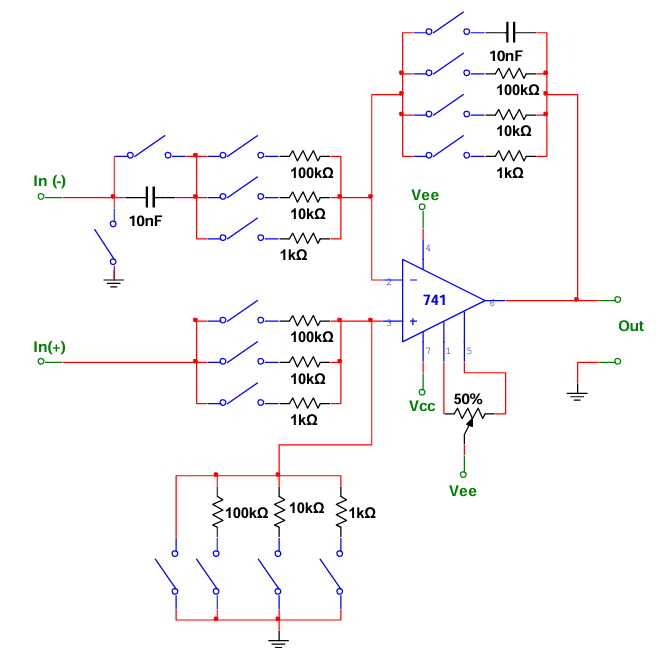
\includegraphics[width=0.47\textwidth]{Placa 1.png}
  \caption{Placa 1 y sus posibles configuraciones}
  \label{fig:placa1}
\end{figure}


\subsubsection{Integrador Operacional}
Se conectó, mediante jumpers, los correspondientes terminales para que se forme el circuito de la \textit{Figura 6}. Se conectó a la entrada el generador de señales y un par de puntas del osciloscopio, y a la salida el otro par. La conexión resultante se observa la imagen de la \textit{Figura 7}:
\begin{figure}[H]
  \centering
  \begin{circuitikz}
        \draw (0,0) node[op amp] (opamp) {}
        (opamp.-) to[short,-] (-2,0.5)
        to[short,*-] (-2,2)
        to[C, l=$10nF (C)$] (1.2,2)
        to[short,*-] (opamp.out);
        
        \draw (-2,0.5) to[R, l_=$1k\Omega (R_1)$] (-4,0.5)
        to[sV, l=$V_e$] (-4,-2.5)
        node[ground]{};
        
        \draw (opamp.+) to[short] (-1.5,-0.5)
        to[short,-] (-1.5,-0.8)
        to[R, l=$1k \Omega (R_2)$] (-1.5,-2)
        to[short] (-1.5,-2.5)
        node[ground]{};
        
        \draw (opamp.out) to[short,*-o] (2,0)
        node[right]{$V_{\text{s}}$};
        
        \draw (-2,2) to[short,*-] (-2,3.5)
        to[R, l=$10k\Omega (R_3)$] (1.2,3.5)
        to[short,-] (1.2,2);
    \end{circuitikz} \\
    \caption{Integrador Operacional, con los valores utilizados de la Placa 1.}
    \label{Integrador}
    \end{figure}


\begin{figure}[H]
  \centering
  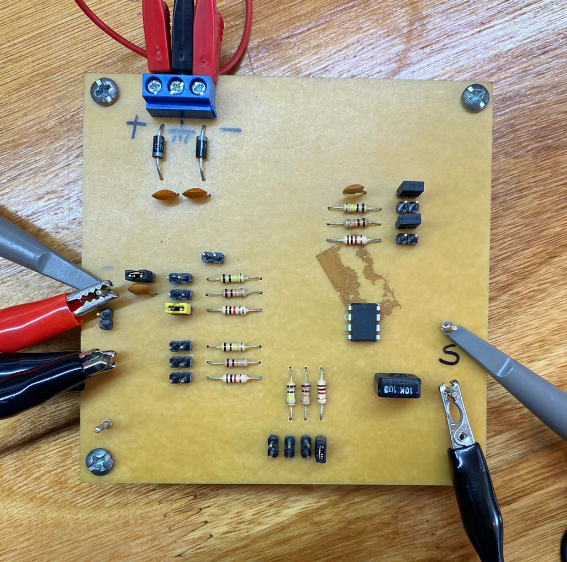
\includegraphics[width=0.47\textwidth]{integrador placa 1/integrador placa 1.png}
  \caption{Placa 1 en configuración de Integrador}
  \label{fig:placa1 integrador}
\end{figure}

Para conocer el comportamiento frecuencial del Circuito Integrador, se observó la salida para entradas de distintas frecuencias.
Se muestran a continuación tres mediciones de osciloscopio para una función Cuadrada de frecuencias $1khz$, $5khz$ y $20kHz$ como entrada:

\begin{figure}[H]
  \centering
  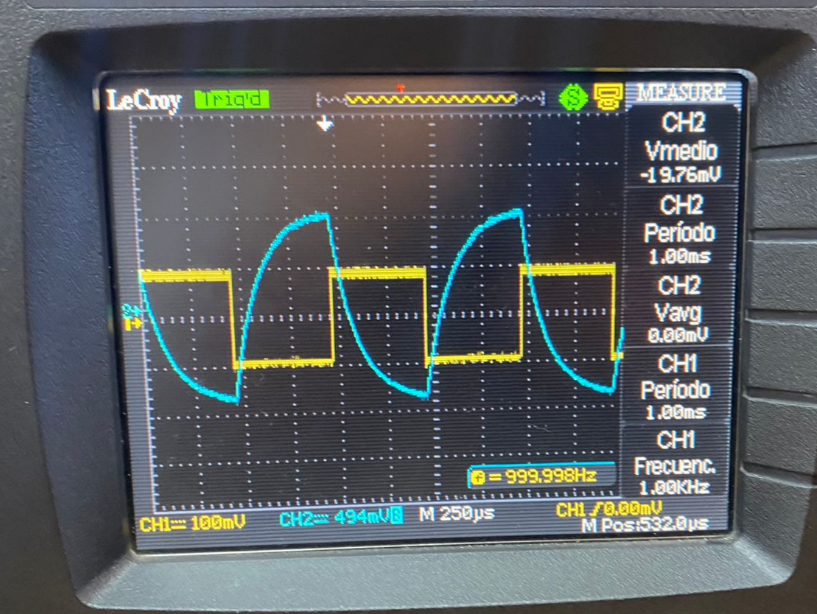
\includegraphics[width=0.47\textwidth]{integrador placa 1/Lectura osciloscopio integrador 1k.png}
  \caption{Medición de Osciloscopio del Integrador Operacional. Entrada en Amarillo, corresponde a una función Cuadrada de frecuencia 1kHz}
  \label{fig:inte1k}
\end{figure}

\begin{figure}[H]
  \centering
  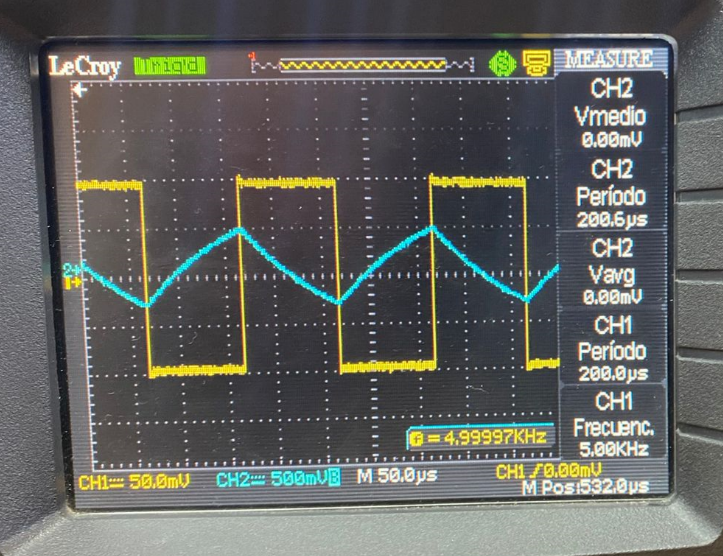
\includegraphics[width=0.47\textwidth]{integrador placa 1/lectura oscioscopio itnegraor 5k.png}
  \caption{Medición de Osciloscopio del Integrador Operacional. Entrada en Amarillo, corresponde a una función Cuadrada de frecuencia 5kHz}
  \label{fig:inte5k}
\end{figure}

\begin{figure}[H]
  \centering
  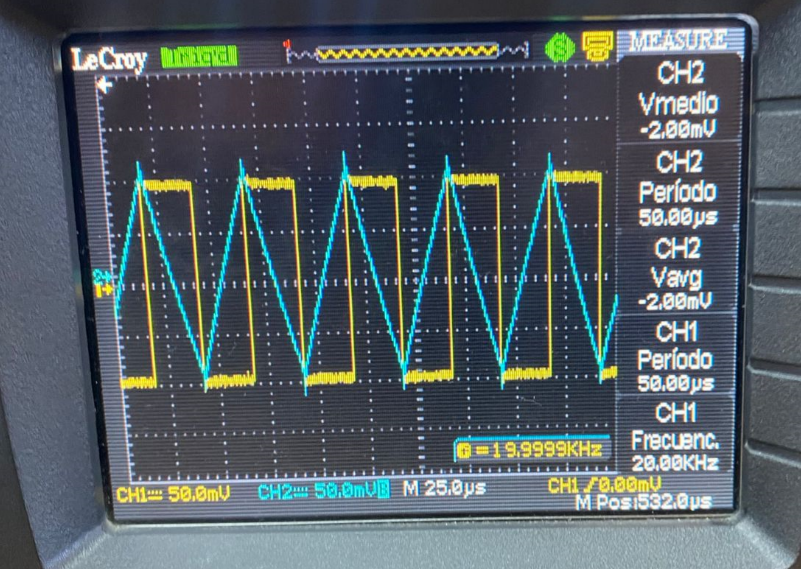
\includegraphics[width=0.47\textwidth]{integrador placa 1/Lectura osciloscopio integrador 20k.png}
  \caption{Medición de Osciloscopio del Integrador Operacional. Entrada en Amarillo, corresponde a una función Cuadrada de frecuencia 20kHz}
  \label{fig:inte20k}
\end{figure}

Pasemos a analizar los resultados.
El integrador deberá tener como salida una función Triángulo para la entrada de la función Cuadrada.\\
Se observa que esto no es cierto para el caso de la entrada de baja frecuencia de $1kHz$, pero sí lo es para la entrada de alta frecuencia de $20kHz$, mientras que para una frecuencia media-baja, de $5kHz$, se obtiene un resultado casi correcto, aunque la salida no es un Triángulo perfecto.\\
Esto se corresponde con lo visto en previamente en la \textit{Sección II: Marco Teórico} acerca de la existencia de un polo. De \textit{(\ref{eq2})}, se tiene:


            \begin{equation}
            A_v =- \frac{-1}{(10nF)(1k\Omega)(s+\frac{1}{(10nF)(10k\Omega)})} \\
            \end{equation}

            \begin{equation}
            A_v =- \frac{-100k}{(s+10k)} \\
            \end{equation}
Por lo que la ubicación del polo es en  $$ s=-10k \rightarrow \textit{f} \approx 1591.54Hz $$

Es por ello que para frecuencias cercanas a $1591Hz$ ($1kHz$, $5kHz$), el funcionamiento del Circuito Integrador no es el deseado, pero sí lo es para frecuencias mucho mayores ($20kHz$).\\
Tener en cuenta que este comportamiento quedó determinado por la ubicación del polo, que está en función de los valores de $R_3$ y $C$.\\

Por último, se realizó un barrido de frecuencia, pero esta vez con una función Triangular en la entrada. Los valores de frecuencia analizados, el proceso y la conclusión es similar al caso de la función cuadrada, por lo que solo se incluirán las imagenes de las tres medidas del osciloscopio. La diferencia notable es que la integración de la función Triángulo da como resultado una función parabóla.

\begin{figure}[H]
  \centering
  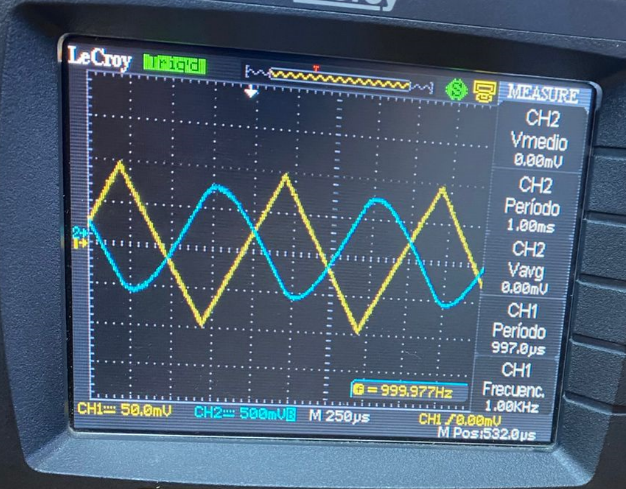
\includegraphics[width=0.47\textwidth]{integrador placa 1/lectura osciloscopio integrador traingulo 1k.png}
  \caption{Medición de Osciloscopio del Integrador Operacional. Entrada en Amarillo, corresponde a una función Triángulo de frecuencia 1kHz. La salida no es la Parábola esperada.}
  \label{fig:inte20k}
\end{figure}

\begin{figure}[H]
  \centering
  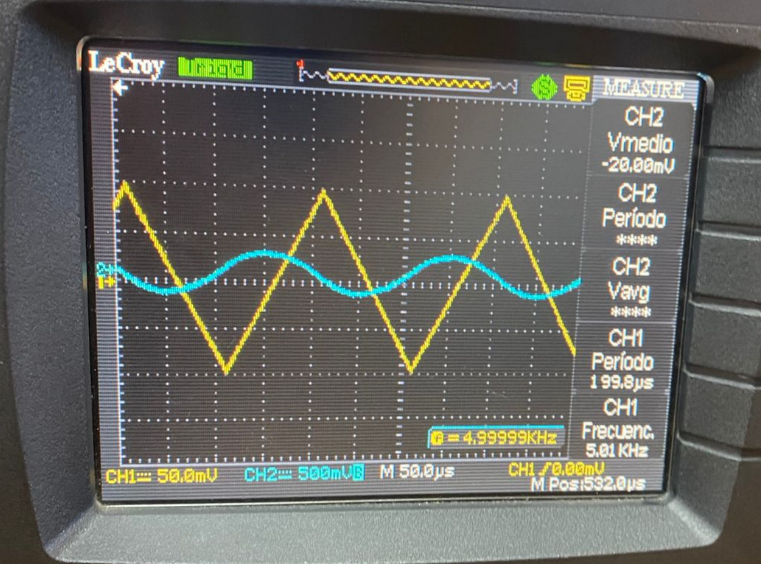
\includegraphics[width=0.47\textwidth]{integrador placa 1/lectura osciloscoio integrador triangulo 5k.png}
  \caption{Medición de Osciloscopio del Integrador Operacional. Entrada en Amarillo, corresponde a una función Triángulo de frecuencia 5kHz. La salida se asemeja mucho a la Parábola.}
  \label{fig:inte20k}
\end{figure}

\begin{figure}[H]
  \centering
  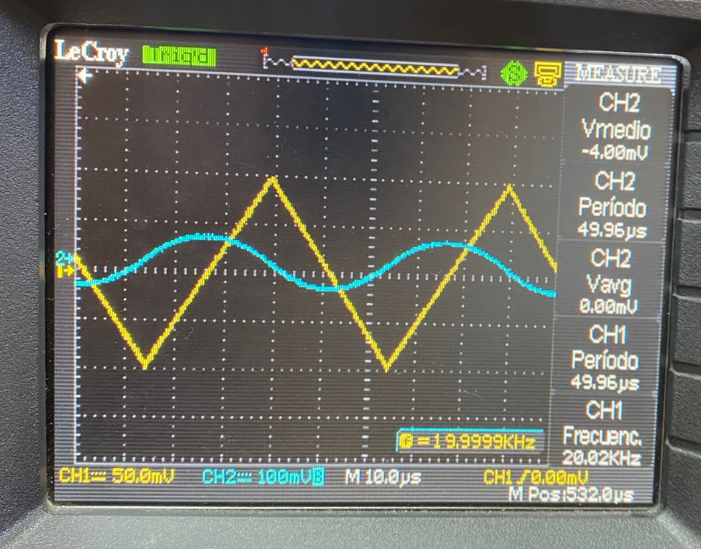
\includegraphics[width=0.47\textwidth]{integrador placa 1/lectura osciloscopio integrador triangulo 20k.png}
  \caption{Medición de Osciloscopio del Integrador Operacional. Entrada en Amarillo, corresponde a una función Triángulo de frecuencia 20kHz. La salida es una Parábola.}
  \label{fig:inte20k}
\end{figure}


\subsubsection{Derivador Operacional}

Se utilizó nuevamente la \textit{Placa 1} para el estudio del Derivador Operacional, esta vez conectada según la configuración y los valores mostrados en la \textit{Figura 14}. El resultado se observa en la imagen de la \textit{Figura 15}.

\begin{figure}[H]
  \centering
  \begin{circuitikz}
    \node[op amp] (opamp) at (0,0) {};
    \draw (opamp.+)-- ++ (-0.3,0) -- ++(0,-0.5) to[R=$10k\Omega(R_2)$] ++ (0,-1.5) node[ground]{};
    \draw (opamp.-) -- ++(-0.5,0) to[R,l_=$1k\Omega(R_1)$] ++(-1.25,0) -- ++(-0.5,0) to[C,l_=$10nF(C)$] ++(-1,0) -- ++(0,-1) to[sV, l=$V_e$] ++(0,-1) -- ++ (0,-1) node[ground]{};
    \draw (opamp.out) -- ++(0.25,0) -- ++(0,2) -- ++(0,0) to[R,l_=$10k\Omega(R_3)$] ++(-2.7,0) -- ++(0,-1.5) node[circ]{};
    \draw (opamp.out) -- ++(0.25,0) node[circ]{} -- ++(0.25,0) node[ocirc]{} coordinate (Vout) node[right] {$V_s$};
  \end{circuitikz}
  \caption{Derivador Operacional}
  \label{diagAODerivador}
\end{figure}

\begin{figure}[H]
  \centering
  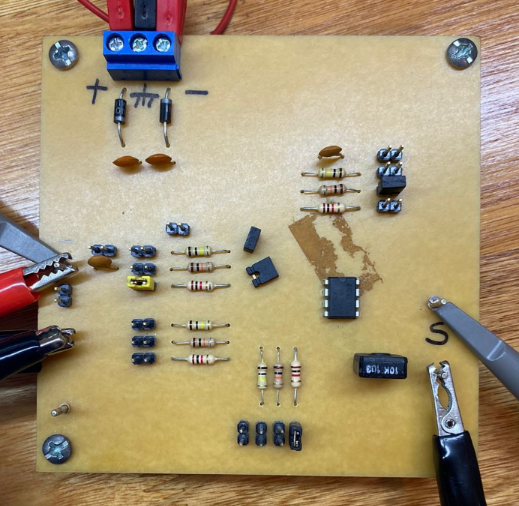
\includegraphics[width=0.47\textwidth]{derivador placa 1/dar vuelta derivador placa 1.png}
  \caption{Placa 1 en configuración de Derivador.}
  \label{fig:derivadorplaca1}
\end{figure}

Se propuso determinar el rango de operación mediante un barrido de frecuencia y observando la salida. \\
Se inyectó una señal Triangulo a la entrada, variando su frecuencia.
A continuación se muestran tres mediciones de osciloscopio, para entradas de $100Hz$, $1kHz$ y $20kHz$.

\begin{figure}[H]
  \centering
  \includegraphics[width=0.47\textwidth]{derivador placa 1/osc derivador cuadrada 100hz.png}
  \caption{Medición de Osciloscopio del Derivador Operacional. Entrada en Amarillo, corresponde a una señal Triangulo de frecuencia $100Hz$.}
  \label{fig:derivadorplaca1}
\end{figure}

\begin{figure}[H]
  \centering
  \includegraphics[width=0.47\textwidth]{derivador placa 1/osc derivador cuadrada 1khz.png}
  \caption{Medición de Osciloscopio del Derivador Operacional. Entrada en Amarillo, corresponde a una señal Triangulo de frecuencia $1kHz$.}
  \label{fig:derivadorplaca1}
\end{figure}

\begin{figure}[H]
  \centering
  \includegraphics[width=0.47\textwidth]{derivador placa 1/osc derivador cuadrada 20khz.png}
  \caption{Medición de Osciloscopio del Derivador Operacional. Entrada en Amarillo, corresponde a una señal Triangulo de frecuencia $20kHz$.}
  \label{fig:derivadorplaca1}
\end{figure}

Para este análisis se utilizó una señal Triángulo, siendo su derivada una señal Cuadrada.\\
Para el caso de baja frecuencia, de $100Hz$, la salida del circuito se corresponde perfectamente con lo esperado: una señal Cuadrada.\\
Para una frecuencia un poco mayor, de $1kHz$ (1 década después), se sigue conservando la forma Cuadrada pero levemente distorsionada, por lo que $1kHz$ no es la frecuencia de operación más deseable.\\
Finalmente, para una frecuencia mayor, de $20kHz$, el circuito claramente ya no se comporta como un Derivador.\\
Esto se corresponde con la ubicación del polo del derivador; según visto en la \textit{Sección II: Marco Teórico, II-B} y reemplazando los valores de resistencias y capacitores en la ecuación \textit{(\ref{eq6})}, se tiene:

            \begin{equation}
            A_v =-\frac{-s10k\Omega}{1k\Omega(s+\frac{1}{(10nF)(1k\Omega)})}  \\
            \end{equation}

            \begin{equation}
            A_v =-\frac{-s10k\Omega}{(s+100k)}  \\
            \end{equation}

Este derivador tiene un cero en el origen (lo cuál es correcto, pues la derivada de una señal constante es cero), y un polo en: $$ s=-100k \rightarrow \textit{f} \approx 15,915 kHz $$

Es por ello que a frecuencias como mínimo una década menos que las del polo ($100Hz$, $1kHz$), el derivador opera correctamente, mientras que a frecuencias cercanas o posteriores a las del polo ($20kHz$), la salida ya no es la adecuada.


\subsection{Placa 2, Amplificador de Instrumentación}

Para el armado y conexión de la placa 2, se procedió según el esquema de la \textit{Figura 20}. La polarización de los AO es de \textit{12V}.

\begin{figure}[H]
  \centering
  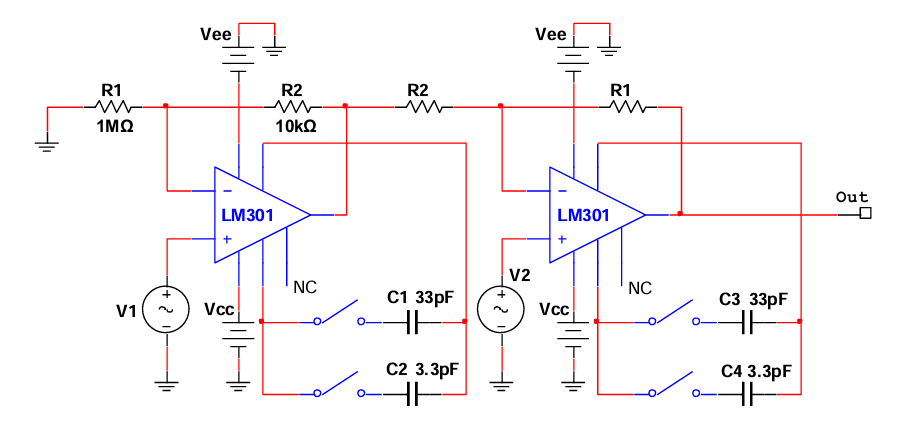
\includegraphics[width=0.47\textwidth]{placa 2/diagrama placa 2.png}
  \caption{Diagrama Completo de la Placa 2.}
  \label{fig:diagramaplaca2}
\end{figure}

Como se observa, los valores de las resistencias son fijos.\\ Existen tambien dos pares de capacitores de compensación. En los primeros estudios, se utilizó el par de capacitores de $3.3pF$ para todas las pruebas. Para los estudios posteriores, se pretende variar los valores de capacitancia para medir el comportamiento en frecuencia de los AO.\\
Nuevamente, se conectó un par de pinzas del osciloscopio a la entrada $V_1$, junto con el generador de funciones; mientras que a la salida se conectó el otro par de pinzas.


\begin{figure}[H]
  \centering
  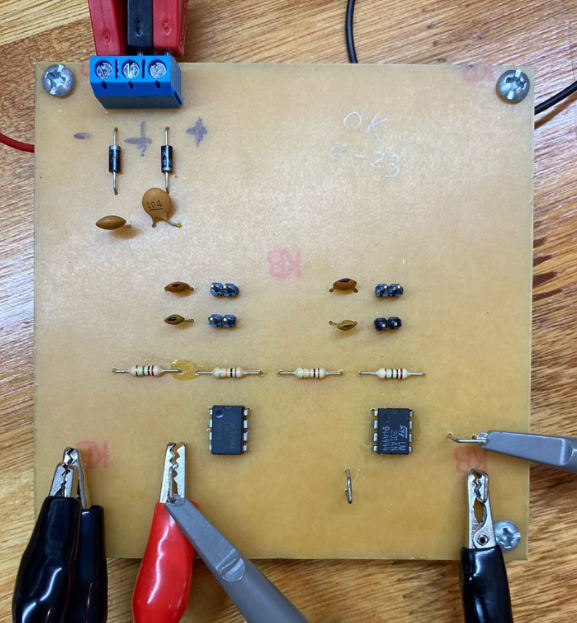
\includegraphics[width=0.47\textwidth]{placa 2/placa 2 sin chumpers.png}
  \caption{Imagen de la Placa 2. No se encuentran colocados los jumpers aún.}
  \label{fig:fotoplaca2}
\end{figure}




\subsection{Placa 2, Entrada $V_1$} %3
Se inyectó con el generador de señal una onda sinusoidal a la entrada $V_1$, con una amplitud $V_{pp}$ de $20mV$, de manera que no haya saturación en la salida, y de frecuencia $100Hz$. La entrada $V_2$ se conectó a tierra.\\

Según la \textit{Figura 19}, la señal deberá pasar por la etapa 1 sin modificación de amplitud ni fase, y luego entrar tal cual a la etapa 2 por el terminal inversor.
En esta etapa, la señal se verá amplificada y desfasada 180°.\\
Según lo visto en la Sección II-C, de \textit{(\ref{eq11})}, la ganancia esperada es:


            \begin{equation}
            A_v =1 + \frac{1M\Omega}{10k\Omega} =  101
            \end{equation}
            
Mientras que la lectura del osciloscopio marca:

\begin{figure}[H]
  \centering
  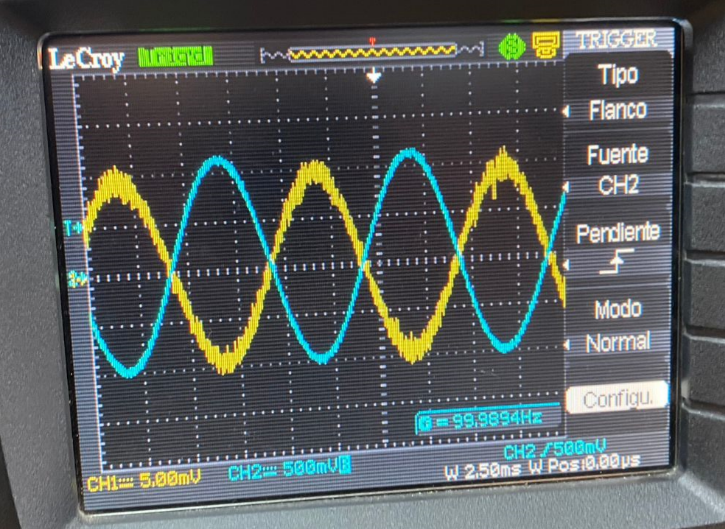
\includegraphics[width=0.47\textwidth]{placa 2/punto 4 osc.png}
  \caption{Lectura del osciloscopio. Entrada en Amarillo. Compensación con capacitores de $3.3pF$ }
  \label{fig:fotoplaca2}
\end{figure}

La ganancia medida es de aproximadamente 100 veces y se corresponde con la ganancia esperada.\\
El desfasaje observado es de 180°, y se corresponde con lo esperado..\\

\subsection{Placa 2, Entrada $V_2$} %4

A continuación se conectó el generador de funciones y se inyecto nuevamente una señal de $20mV V_{pp}$ y frecuencia $100Hz$, esta vez en la entrada $V_2$, mientras que la entrada $V_1$ se conectó a tierra.\\

Nuevamente la ganancia esperada es la de la etapa 2:

\begin{equation}
            A_v =1 + \frac{1M\Omega}{10k\Omega} =  101
            \end{equation}

A diferencia del caso anterior, la señal se inyecta por la entrada no inversora, por lo que se espera un desfasaje nulo.\\


\begin{figure}[H]
  \centering
  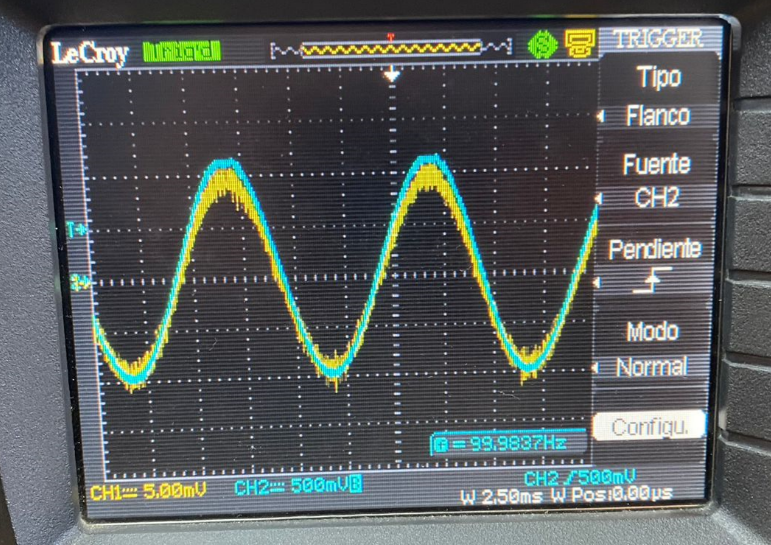
\includegraphics[width=0.47\textwidth]{placa 2/punto3 osc .png}
  \caption{Lectura del osciloscopio. Entrada en Amarillo, muestra una ganancia aproximada de 100 veces. El desfasaje es nulo. Compensación con capacitores de $3.3pF$ }
  \label{fig:fotoplaca2}
\end{figure}

Las lecturas de osciloscopio se corresponden con lo esperado.


\subsection{Compensación en Frecuencia} 
El objetivo de esta sección es conocer la ubicación del polo dominante, en función de los capacitores utilizados para su compensación. \\
Para ello se realizó un barrido de frecuencia con una señal sinusoidal de $Vpp$ $20mV$ inyectada en $V_1$.\\
Con el barrido de frecuencias se pretendió encontrar una atenuación de $3dB$ en la salida, indicando así la ubicación del polo.


\subsubsection{Capacitores de $33pF$} 
Se colocaron jumpers en la Placa 2, de manera que queden conectados los capactiores de $33pF$.\\
A continuación se realizó el barrido de frecuencia. El valor que corresponde a una atenuación de $3db$ para la señal de $20mV$ es:

            \begin{equation}
            \frac{20mV}{\sqrt{2}} \approx 14.14mV 
            \end{equation}

\begin{figure}[H]
  \centering
  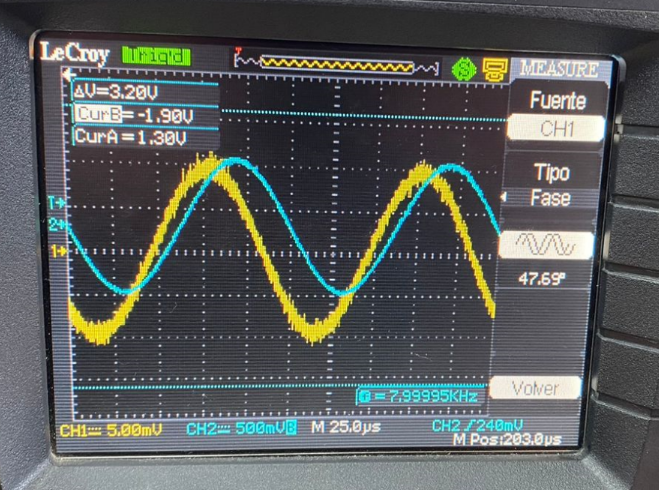
\includegraphics[width=0.47\textwidth]{placa 2/frecuencia polo placa 2 3coma3.png}
  \caption{La frecuencia medida para la atenuación de $3dB$ fue de $8.5kHz$. Compensación con capacitores de $33pF$ }
  \label{fig:fotoplaca2}
\end{figure}

La ubicación del polo, y por lo tanto la frecuencia de corte superior, es $8.5kHz$ utilizando los capacitores de $33pF$ . \\Tener en cuenta que para una medición más clara con el osciloscopio, se eligió una escala adecuada para ignorar la ganancia de 101 veces producto de la etapa 2.

\subsubsection{Capacitores de $3.3pF$} 
Se colocaron jumpers en la Placa 2, de manera que queden conectados los capactiores de $3.3pF$.\\
A continuación se realizó el barrido de frecuencia. El valor que corresponde a una atenuación de $3db$ para la señal de $20mV$ es:

            \begin{equation}
            \frac{20mV}{\sqrt{2}} \approx 14.14mV 
            \end{equation}

\begin{figure}[H]
  \centering
  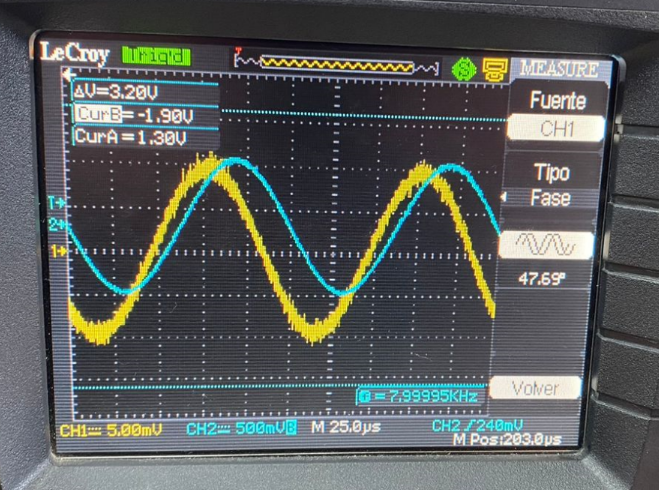
\includegraphics[width=0.47\textwidth]{placa 2/frecuencia polo placa 2 3coma3.png}
  \caption{Se observa una amplitud aproximada de 15. La frecuencia medida para la atenuación de $3dB$ fue de $27kHz$. Compensación con capacitores de $3.3pF$ }
  \label{fig:fotoplaca2}
\end{figure}

La ubicación del polo, y por lo tanto la frecuencia de corte superior, es $27kHz$ utilizando los capacitores de $3.3pF$ . \\Tener en cuenta que para una medición más clara con el osciloscopio, se eligió una escala adecuada de modo que se pueda ignorar gráficamente la ganancia de 101 veces producto de la etapa 2.


\begin{table}[h]
\begin{center}
\begin{tabular}{|c||c|}
\hline
Capacitores & Frecuencia de corte\\
\hline
3.3pF & 27kHz\\
\hline
33pF & 8.5kHz\\
\hline
\end{tabular}
\end{center}
\caption{Mediciones de compensación}
\label{tab:simple}
\end{table}

\subsection{Modo Común - Ganancia}

\begin{figure}[H]
  \centering
  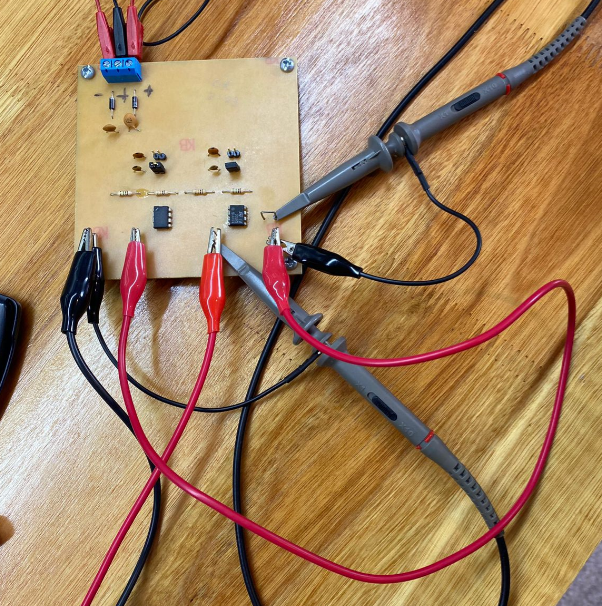
\includegraphics[width=0.47\textwidth]{modo comun/modo comun.png}
  \caption{La fuente de señal está conectada a $V_1$ y $V_2$ en simultáneo. }
  \label{fig:fotoplaca2}
\end{figure}

\begin{figure}[H]
  \centering
  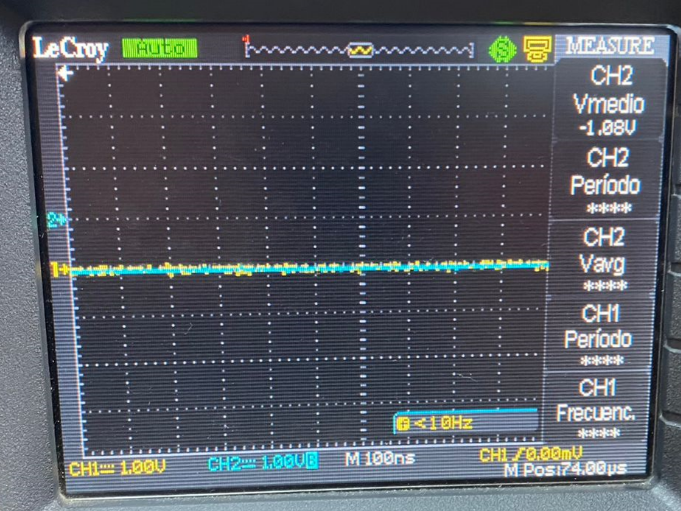
\includegraphics[width=0.47\textwidth]{modo comun/cmrr.png}
  \caption{Entrada en Amarillo, Salida en Azul.  }
  \label{fig:cmrr}
\end{figure}

Observando la etapa 2, se esperaba una amplificación de la diferencia entre $V_2$ y $V_1$, y un rechazo a las señales comunes.\\
Al tener la misma señal para ambas entradas, la diferencia medida fué cero en el osciloscopio \textit{(Figura 26)}.\\
Con respecto al ruido que pueden contener cualquiera de las dos señales, se debe ver amplificado (siempre y cuando no sea común a ambas entradas).




\section{Conclusiones}

Los experimentos realizados permitieron verificar el comportamiento teórico de los circuitos integrador y derivador operacionales. Se comprobó que ambos circuitos tienen un rango de operación adecuado, determinado por la ubicación de sus polos. En el caso del integrador, se obtuvo la salida esperada a frecuencias altas, mientras que para el derivador, a frecuencias bajas. El amplificador de instrumentación demostró la capacidad de compensar sus polos, y a su vez sirvió para mostrar un rechazo al modo común.\\
Todas las mediciones y pruebas fueron las esperadas según calculos teóricos previos y se condicen con lo visto en el \textit{Marco Teórico}.
 

\addtolength{\textheight}{-12cm}   % This command serves to balance the column lengths
                                  % on the last page of the document manually. It shortens
                                  % the textheight of the last page by a suitable amount.
                                  % This command does not take effect until the next page
                                  % so it should come on the page before the last. Make
                                  % sure that you do not shorten the textheight too much.

%%%%%%%%%%%%%%%%%%%%%%%%%%%%%%%%%%%%%%%%%%%%%%%%%%%%%%%%%%%%%%%%%%%%%%%%%%%%%%%%



%%%%%%%%%%%%%%%%%%%%%%%%%%%%%%%%%%%%%%%%%%%%%%%%%%%%%%%%%%%%%%%%%%%%%%%%%%%%%%%%



%%%%%%%%%%%%%%%%%%%%%%%%%%%%%%%%%%%%%%%%%%%%%%%%%%%%%%%%%%%%%%%%%%%%%%%%%%%%%%%%



%\section*{ACKNOWLEDGMENT}

%The preferred spelling of the word Òacknowledgment\'o in America is without an Òe\'o after the Òg\'o. Avoid the stilted expression, ÒOne of us (R. B. G.) thanks . . .\'o  Instead, try ÒR. B. G. thanks\'o. Put sponsor acknowledgments in the unnumbered footnote on the first page.



%%%%%%%%%%%%%%%%%%%%%%%%%%%%%%%%%%%%%%%%%%%%%%%%%%%%%%%%%%%%%%%%%%%%%%%%%%%%%%%%


\begin{thebibliography}{99}

\bibitem{c1} J. Millman and A. Grabel, ``Microelectrónica,” McGraw-Hill, New York, 6ta edición, 1993.
\bibitem{c2} P. R. Gray and R. G. Meyer, ``Analysis and Design of Analog Integrated Circuits,” John Wiley & Sons, New York, 4th edition, 2001



\end{thebibliography}




\end{document}
